\documentclass[11pt]{article}

\usepackage[margin=0.78in]{geometry}
\usepackage{amsmath}
\usepackage{amssymb}
\usepackage{booktabs}
\usepackage{graphicx}
\usepackage{hyperref}
\usepackage{microtype}
\usepackage{caption}
\usepackage{xcolor}

\hypersetup{
    colorlinks=true,
    linkcolor=black,
    citecolor=blue!60!black,
    urlcolor=blue!60!black
}

\title{\vspace{-1.0cm}A Pair-Correlation Descriptor for Sampling Ce/Zr Configuration Space in Ceria-Doped Zirconia}
\author{M. Waseem Ashraf}
\date{\today}

\begin{document}
\maketitle

\begin{abstract}
Sampling cation configurations in ceria-doped zirconia requires a descriptor that is tied to the substitutional degrees of freedom before relaxation, yet remains interpretable after first-principles response calculations.  We show that shell-resolved Ce/Zr pair correlations provide such a descriptor.  Assigning an Ising-like occupation variable $\sigma_i=+1$ for Ce and $\sigma_i=-1$ for Zr on each cation site, each starting structure is represented by the average product $\langle\sigma_i\sigma_j\rangle$ over cation pairs in a distance shell.  Principal-component analysis of these vectors separates the 16 calculated POSCAR configurations into four regions of Ce/Zr ordering space.  Representative configurations selected from these regions, POSCAR.7, POSCAR.14, POSCAR.2, and POSCAR.4, span distinct relaxed dielectric, soft-mode, and lattice-distortion responses.  The descriptor is therefore appropriate for publishable configuration-space sampling: it should be used to demonstrate coverage of cation-ordering motifs, while dielectric trends should be presented as response overlays rather than as a stand-alone predictive model.
\end{abstract}

\section*{Motivation}
Ceria-doped zirconia is a configurational problem on a cation sublattice: at fixed composition, different Ce/Zr arrangements generate different local strain fields, oxygen relaxations, phonon softening, and ionic dielectric tensors.  A sampling descriptor should therefore satisfy three conditions.  First, it must be defined on the starting configuration, before geometry relaxation or expensive density-functional perturbation theory (DFPT).  Second, it must distinguish local cation order rather than only global composition.  Third, it should be mathematically compatible with established configurational-alloy methods.

Cluster-correlation functions meet these requirements.  They are the standard coordinates of cluster expansions for substitutional alloys and ionic materials \cite{sanchez2017,zhang2016,barroso2024,barroso2022}.  In the present data set, the pair-correlation descriptor is also more appropriate for sampling than soft-mode or dielectric descriptors, because phonon and dielectric quantities are outcomes of the calculation rather than independent sampling coordinates.

\section*{Descriptor}
For a binary Ce/Zr cation sublattice, define the occupation variable
\begin{equation}
    \sigma_i =
    \begin{cases}
        +1, & \text{site } i \text{ occupied by Ce},\\
        -1, & \text{site } i \text{ occupied by Zr}.
    \end{cases}
\end{equation}
For each pair shell $s$, the shell-averaged pair correlation is
\begin{equation}
    \Pi_s =
    \frac{1}{N_s}
    \sum_{i<j}
    \Theta_s(d_{ij})\,\sigma_i\sigma_j ,
    \label{eq:paircorr}
\end{equation}
where $d_{ij}$ is the minimum-image cation--cation distance, $\Theta_s(d_{ij})=1$ when the pair belongs to shell $s$ and $0$ otherwise, and $N_s=\sum_{i<j}\Theta_s(d_{ij})$.  In this work, shells were binned at 0.25~\AA{} and near-zero duplicate/self-like distances were removed.  A value $\Pi_s=+1$ indicates like-cation enrichment in shell $s$; $\Pi_s=-1$ indicates Ce--Zr enrichment; and $\Pi_s\approx0$ indicates a mixed shell.  Each structure is represented by the vector
\begin{equation}
    \boldsymbol{\Pi} = \left(\Pi_{s_1},\Pi_{s_2},\ldots,\Pi_{s_m}\right).
\end{equation}
The descriptor is intentionally low-order.  Pair correlations are easier to interpret and more robust for a 16-structure data set than triplet or quadruplet vectors, whose feature spaces are sparse.  Higher-order clusters remain useful for later cluster-expansion fitting, but they are not the most defensible primary sampling coordinate at this data size.

\section*{Configuration-Space Map}
The pair-correlation vectors were standardized and projected by principal-component analysis (PCA).  The first two principal components explain 36.5\% of the variance and separate the structures into four regions of Ce/Zr ordering space.  Deterministic $k$-means clustering in the PC1--PC2 plane selected one representative structure nearest each cluster centroid.

\begin{figure}[h!]
    \centering
    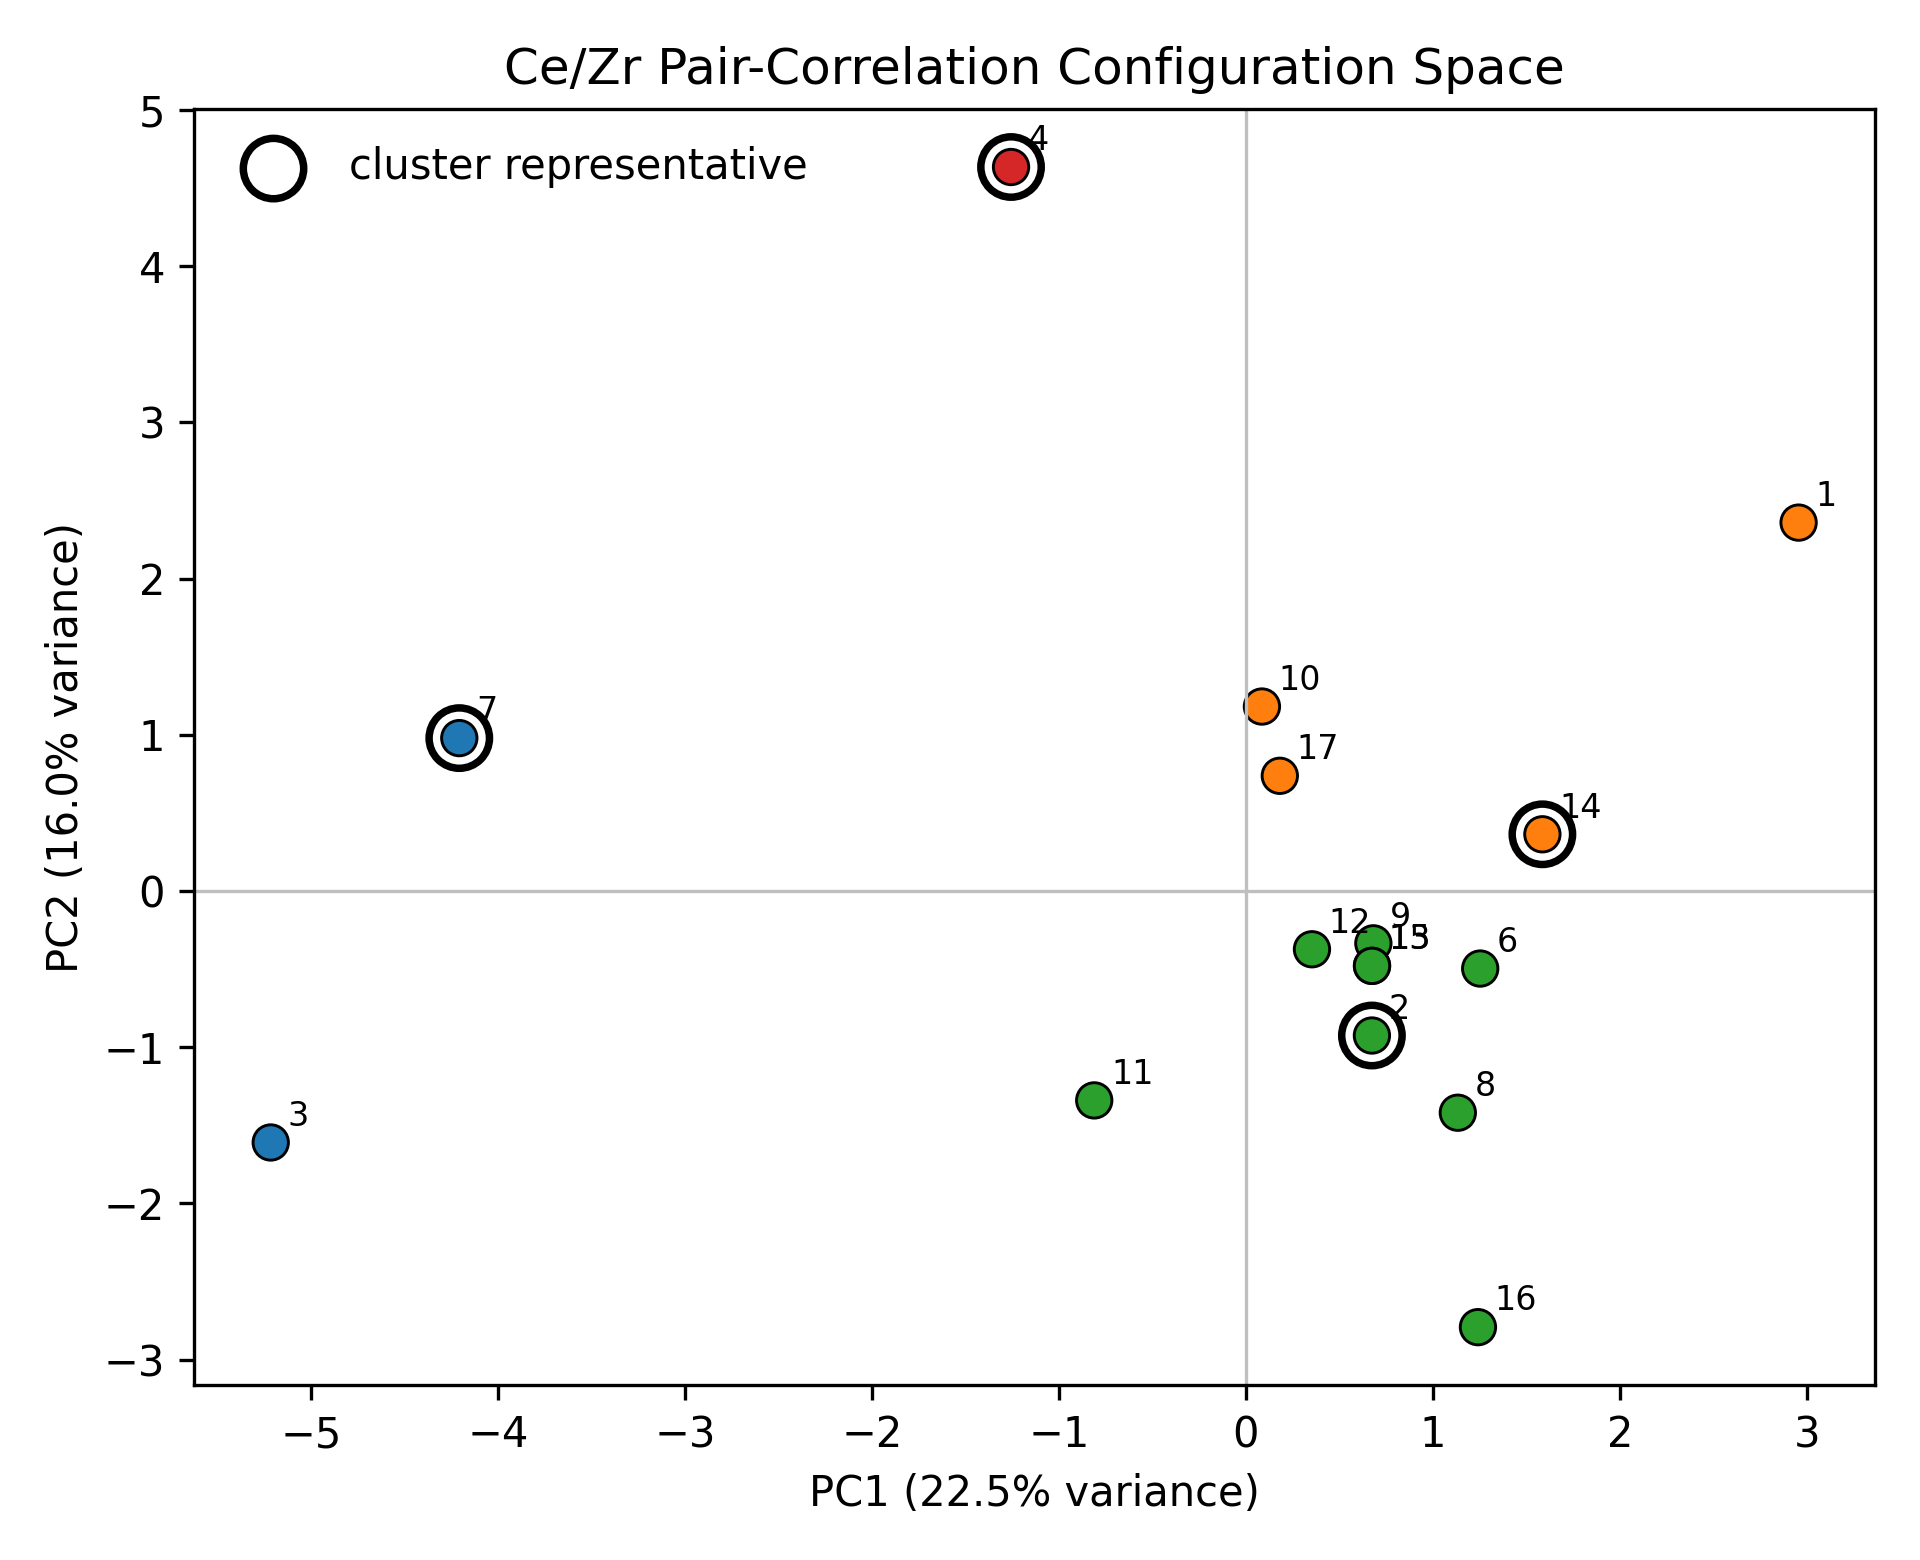
\includegraphics[width=0.82\textwidth]{../configuration_sampling_results/configuration_space_pca_clusters.png}
    \caption{PCA map of shell-binned Ce/Zr pair-correlation vectors.  Circled structures are cluster representatives selected from the pair-correlation configuration space.  The representatives are POSCAR.7, POSCAR.14, POSCAR.2, and POSCAR.4.}
    \label{fig:pca}
\end{figure}

\begin{table}[h!]
\centering
\caption{Representative structures selected from the pair-correlation configuration-space clusters.}
\begin{tabular}{lrrrr}
\toprule
Representative & Cluster & PC1 & PC2 & $\mathrm{Tr}(\epsilon_\mathrm{ion})/3$ \\
\midrule
POSCAR.7  & 1 & -4.206 &  0.979 & 41.391 \\
POSCAR.14 & 2 &  1.585 &  0.363 & 41.533 \\
POSCAR.2  & 3 &  0.673 & -0.925 & 44.286 \\
POSCAR.4  & 4 & -1.256 &  4.635 & 44.468 \\
\bottomrule
\end{tabular}
\label{tab:representatives}
\end{table}

The shell-resolved heatmap in Fig.~\ref{fig:heatmap} shows the direct descriptor values behind the PCA map.  This is the most transparent sampling figure because it reports the actual pair-correlation vector rather than only its reduced coordinates.

\begin{figure}[h!]
    \centering
    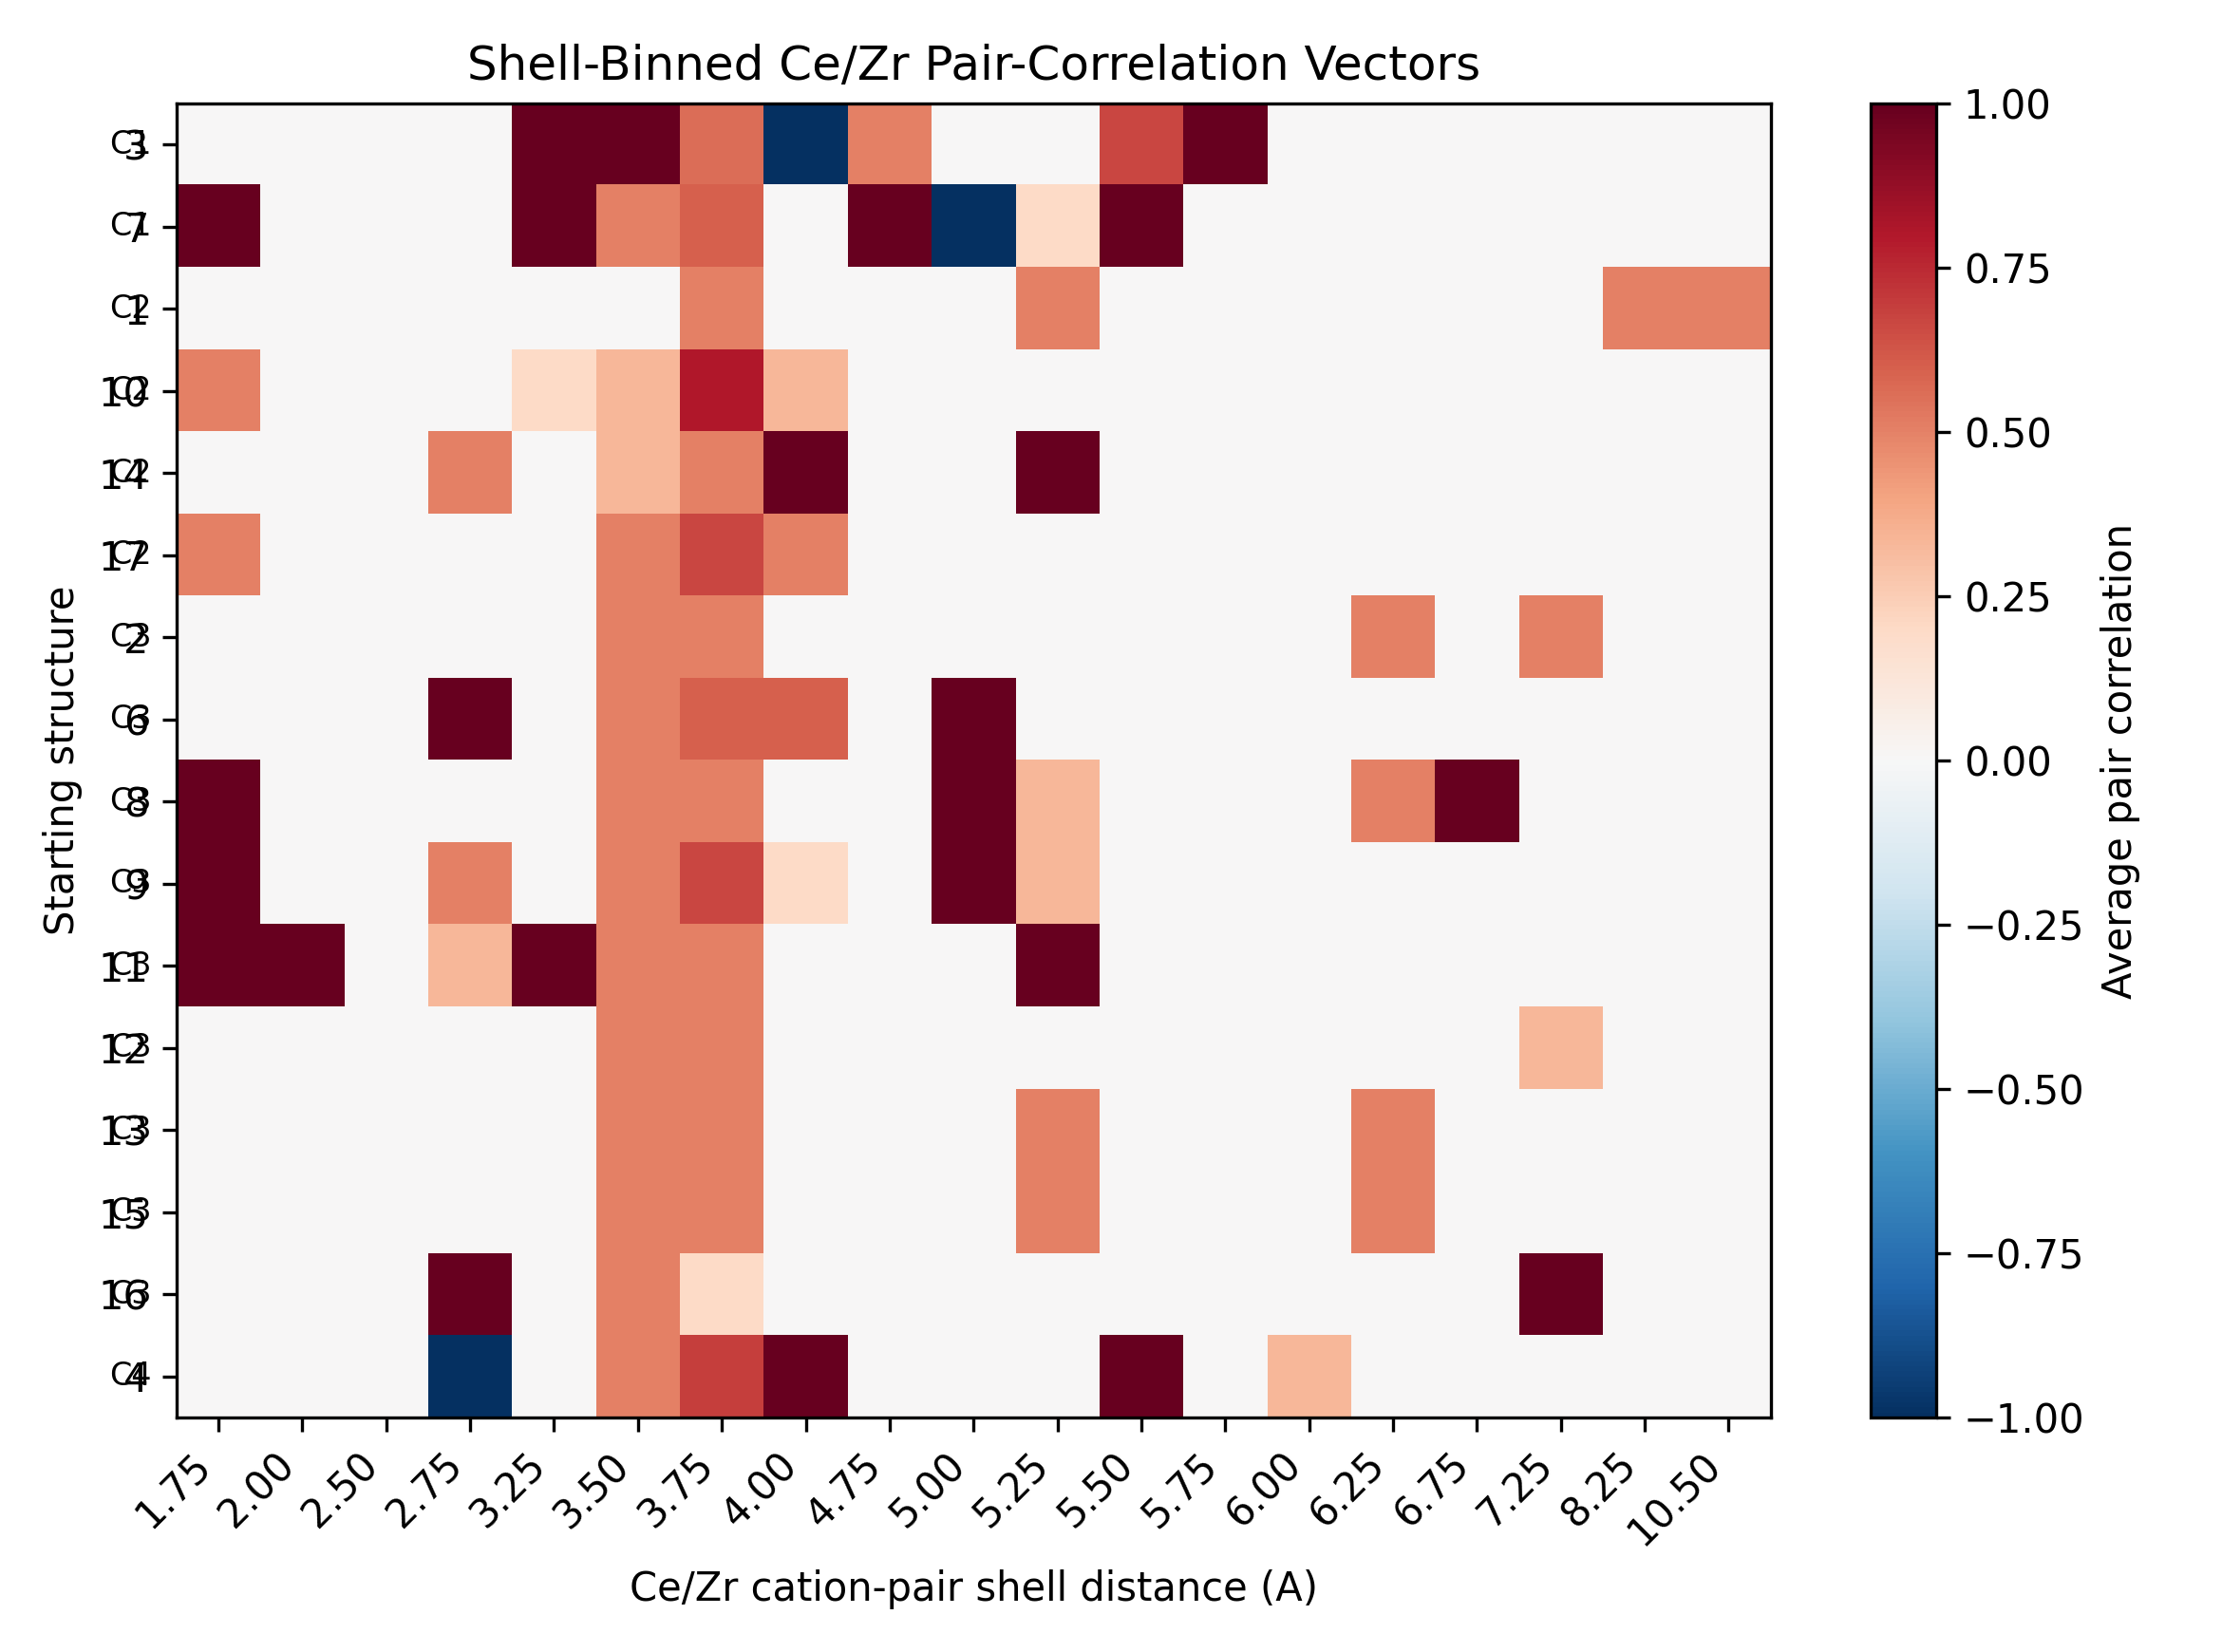
\includegraphics[width=0.90\textwidth]{../configuration_sampling_results/pair_correlation_shell_heatmap.png}
    \caption{Shell-binned Ce/Zr pair-correlation vectors grouped by configuration-space cluster.  Positive values indicate like-cation correlations, negative values indicate Ce--Zr correlations, and values near zero indicate mixed local order.}
    \label{fig:heatmap}
\end{figure}

\section*{Connection to Dielectric Response}
The descriptor in Eq.~\ref{eq:paircorr} is a sampling descriptor, not a direct dielectric model.  This distinction is important.  Ionic dielectric response is governed by phonon mode oscillator strengths divided by squared phonon frequencies; in DFPT form, the ionic susceptibility can be written schematically as
\begin{equation}
    \chi^{\mathrm{ion}}_{\alpha\beta}
    \propto
    \frac{1}{\Omega}
    \sum_m
    \frac{
    \widetilde{Z}^{*}_{m,\alpha}
    \widetilde{Z}^{*}_{m,\beta}
    }{\omega_m^2},
    \label{eq:dielectric}
\end{equation}
where $\Omega$ is the cell volume, $\omega_m$ is a zone-center phonon frequency, and $\widetilde{Z}^{*}_{m,\alpha}$ is the mode effective charge \cite{polymer2018,quantumatk}.  Recent oxide dielectric machine-learning work also identifies soft optical modes, local geometric distortion, and neighbor-distance variation as important structural indicators of high ionic permittivity \cite{shimano2023}.  Thus, the role of the pair-correlation descriptor is to sample cation order; the role of DFPT response quantities is to test which sampled ordering motifs produce larger dielectric response.

\begin{figure}[h!]
    \centering
    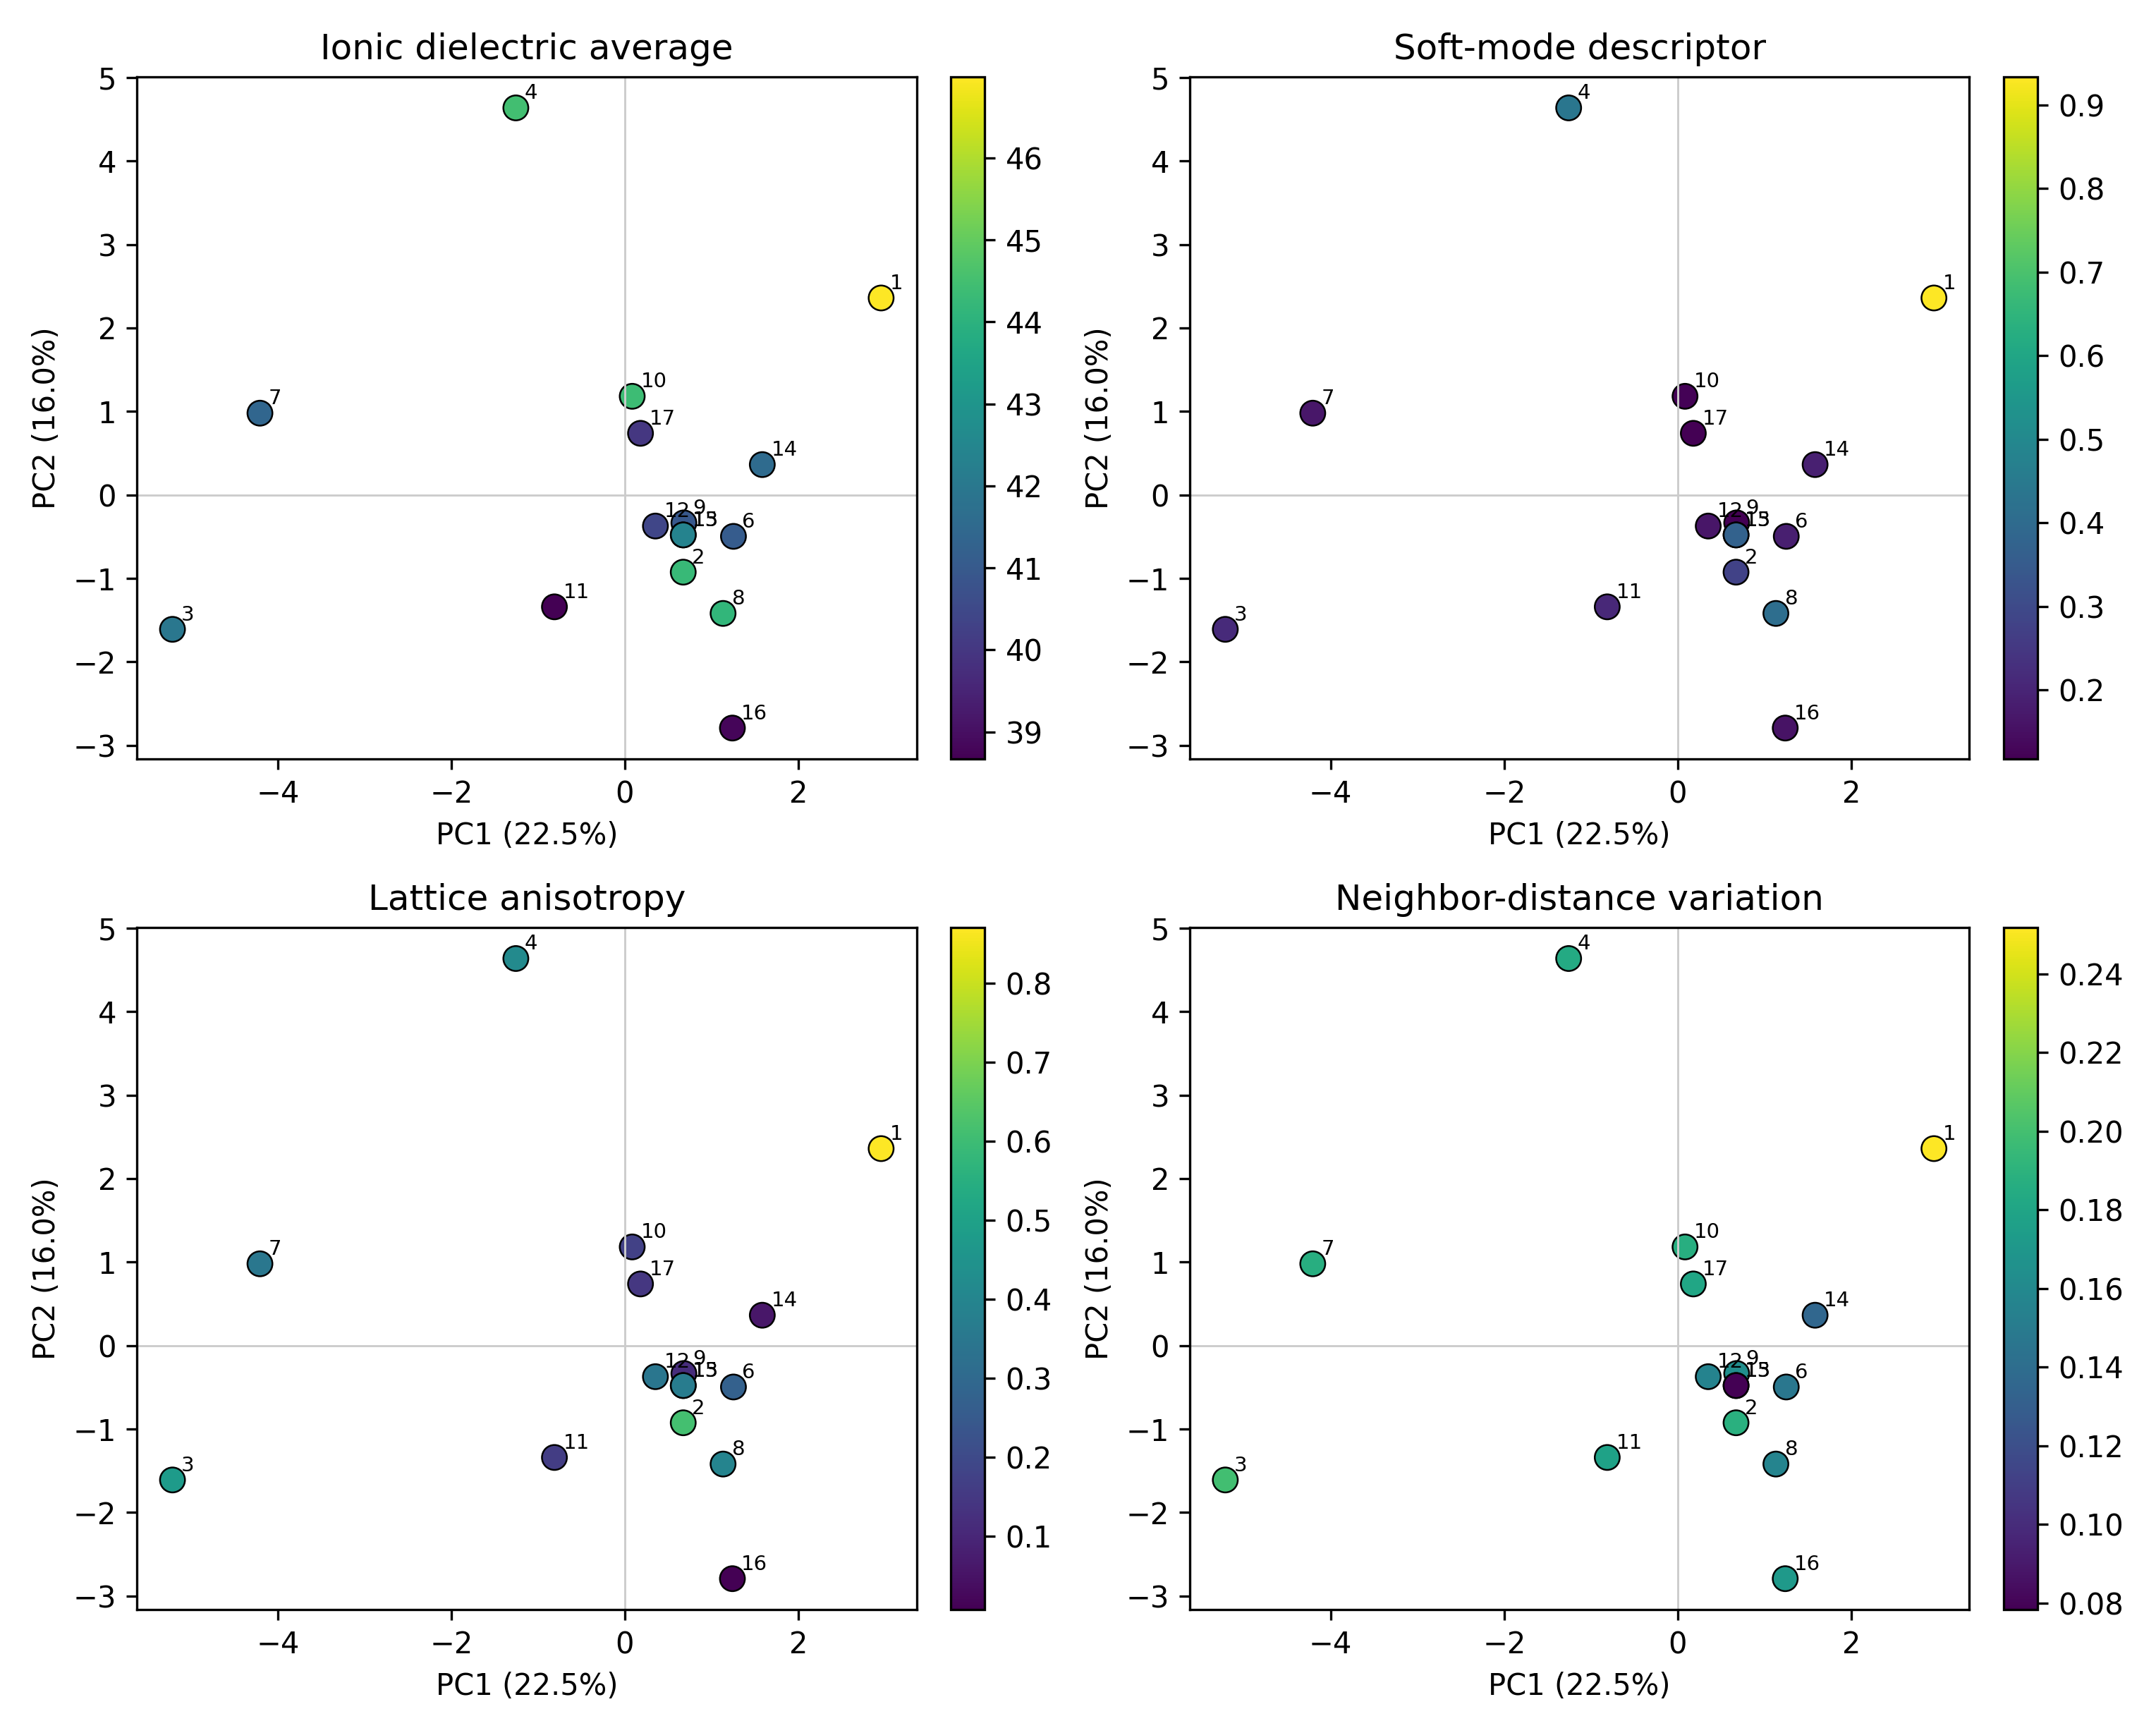
\includegraphics[width=0.95\textwidth]{../configuration_sampling_results/configuration_space_response_overlays.png}
    \caption{Response overlays on the same pair-correlation PCA map.  The four panels show the orientationally averaged ionic dielectric tensor, a soft-mode descriptor $1/\omega_\mathrm{soft}^2$, lattice anisotropy, and mean neighbor-distance variation.  The response variation across the pair-correlation map shows that the descriptor samples physically distinct ordering motifs.}
    \label{fig:overlays}
\end{figure}

Figure~\ref{fig:overlays} shows that different regions of the cation-ordering map produce different dielectric and structural responses after relaxation.  This supports the use of the pair-correlation descriptor for selecting a compact but diverse set of configurations.  It does not claim that the first two PCA coordinates alone predict the dielectric tensor.

\section*{Interpretation}
The reason the descriptor works for sampling is structural.  Ce and Zr occupy the same cation sublattice but impose different local chemical and elastic environments.  Pair correlations measure whether Ce atoms are isolated by Zr, clustered with other Ce, or arranged in longer-range motifs.  Those motifs change the relaxed lattice anisotropy, oxygen displacement field, and soft-mode landscape.  The descriptor therefore connects the controllable configuration variable, cation ordering, to the downstream response variables without using those response variables to choose the sample.

For the present 16-structure data set, a publishable claim should be conservative:
\begin{quote}
Shell-resolved Ce/Zr pair correlations provide a literature-grounded descriptor for sampling cation-ordering configuration space in ceria-doped zirconia.  PCA and clustering of these vectors identify representative configurations that span distinct relaxed dielectric, phonon, and structural responses.
\end{quote}
The stronger claim that pair correlations alone predict the dielectric tensor would require a larger training set and an explicit validation study.

\section*{Conclusion}
Shell-binned Ce/Zr pair correlations are the best descriptor found here for publishable configuration-space sampling.  They are defined before relaxation, encode the relevant cation-ordering degree of freedom, and are grounded in cluster-expansion theory.  In the present data set, the descriptor identifies four representative configurations, POSCAR.7, POSCAR.14, POSCAR.2, and POSCAR.4, that span distinct regions of ordering space and show different ionic dielectric and soft-mode behavior after DFPT.  The recommended workflow is therefore: sample by pair-correlation coverage, then interpret dielectric response by overlaying relaxed lattice, phonon, and dielectric quantities.

\begin{thebibliography}{9}

\bibitem{sanchez2017}
J. M. Sanchez, ``Foundations and Practical Implementations of the Cluster Expansion,'' \emph{Journal of Phase Equilibria and Diffusion} \textbf{38}, 238--251 (2017). \url{https://doi.org/10.1007/s11669-017-0521-3}.

\bibitem{zhang2016}
X. Zhang and M. H. F. Sluiter, ``Cluster Expansions for Thermodynamics and Kinetics of Multicomponent Alloys,'' \emph{Journal of Phase Equilibria and Diffusion} \textbf{37}, 44--52 (2016). \url{https://doi.org/10.1007/s11669-015-0427-x}.

\bibitem{barroso2024}
L. Barroso-Luque and G. Ceder, ``The cluster decomposition of the configurational energy of multicomponent alloys,'' \emph{npj Computational Materials} \textbf{10}, 158 (2024). \url{https://doi.org/10.1038/s41524-024-01338-y}.

\bibitem{barroso2022}
L. Barroso-Luque, P. Zhong, J. H. Yang, F. Xie, T. Chen, B. Ouyang, and G. Ceder, ``Cluster expansions of multicomponent ionic materials: Formalism and methodology,'' \emph{Physical Review B} \textbf{106}, 144202 (2022). \url{https://doi.org/10.1103/PhysRevB.106.144202}.

\bibitem{shimano2023}
Y. Shimano, A. Kutana, and R. Asahi, ``Machine learning and atomistic origin of high dielectric permittivity in oxides,'' \emph{Scientific Reports} \textbf{13}, 22236 (2023). \url{https://doi.org/10.1038/s41598-023-49603-2}.

\bibitem{polymer2018}
R. Ramprasad and co-workers, ``Computational screening of organic polymer dielectrics for novel accelerator technologies,'' \emph{Scientific Reports} \textbf{8}, 9258 (2018). \url{https://pmc.ncbi.nlm.nih.gov/articles/PMC6006378/}.

\bibitem{quantumatk}
Synopsys QuantumATK Documentation, ``DielectricTensor,'' accessed 2026. \url{https://docs.quantumatk.com/manual/Types/DielectricTensor/DielectricTensor.html}.

\end{thebibliography}

\end{document}
